\documentclass[10pt,a4paper]{article}
\usepackage[utf8]{inputenc}
\usepackage[spanish]{babel}
\usepackage{amsmath}
\usepackage{amsfonts}
\usepackage{amssymb}
\usepackage{makeidx}
\usepackage{graphicx}
\usepackage{lmodern}
\usepackage{kpfonts}
\usepackage[left=2cm,right=2cm,top=2cm,bottom=2cm]{geometry}
\begin{document}
\begin{center}

\includegraphics[scale=0.25]{imagenes/upzmg.png} 
\end{center}
\large \huge Fabian canales ochoa, ING. Mecatroica 7-A
\\ \\ 
Aplicaciones de los manipuladores paralelos\\
La principal ventaja de los robots paralelos viene dada por la capacidad de distribuir las cargas
aplicadas sobre el elemento terminal entre las piernas o cadenas cinemáticas abiertas que unen la
plataforma móvil a la plataforma base. Es así como las cadenas cinemáticas o piernas le
proporcionan una mayor rigidez al robot. Sin embargo, las piernas limitan su espacio de trabajo por las
restricciones que introducen la configuración de cadena cerrada.APLICACIONES INICIALES.
Un robot paralelo consiste de una plataforma móvil unida a una plataforma fija mediante una serie
de cadenas cinemáticas llamadas piernas. Partiendo del anterior concepto, Bonev [2] establece que el
origen del robot paralelo se encuentra en la industria del entretenimiento, siendo James E. Gwinnett en
el año 1928 uno de los pioneros en patentar un artefacto basado en el concepto de robot paralelo.
No fue sino hasta 1965 que aparece la primera publicación científica referida a un robot paralelo.
Stewart [8] introduce un robot paralelo de 6 GdL similar al de Gough. Debido al parecido que presenta
la plataforma Stewart con el robot propuesto por Gough hoy en día la configuración del tipo hexápodo
con actuadores lineales se conoce como plataforma Gough-Stewart.
\begin{center}
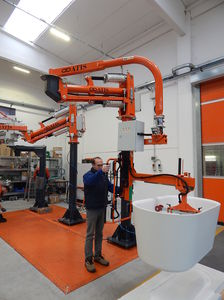
\includegraphics[scale=3.1]{imagenes/aplicacion.png} imagen 4.0
\end{center}
\begin{center}
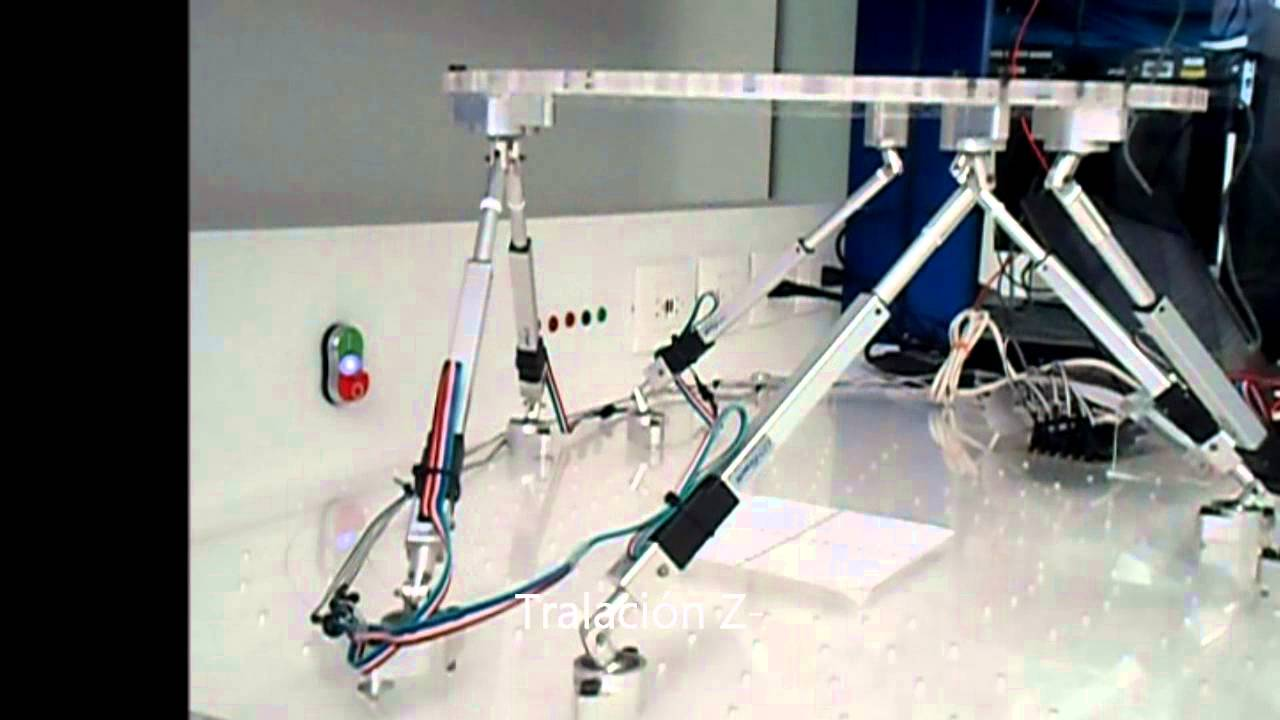
\includegraphics[scale=0.2]{imagenes/33.png} imagen 4.1
\end{center}
APLICACIONES DE PICK AND PLACE (RECOGER Y COLOCAR)
Luego de la introducción de la configuración de robot paralelo para desarrollar simuladores de 
vuelo, la aplicación más conocida y desarrollada de estos robot es en operaciones de pick and place. Es
de destacar que el robot serial equivalente para este tipo de operaciones lo constituye el robot SCARA
(Selective Compliant Assembly Robot Arms) que presenta 4 GdL. Un robot SCARA permite posicionar
el elemento terminal, y por ende la pieza, en el espacio cartesiano, además también puede realizar una
rotación. A este tipo de movimiento se le conoce como movimiento de Schoenflies.
APLICACIONES EN CENTRO DE MECANIZADO.
Otra de las aplicaciones prácticas de los robots paralelos se encuentra en el área de desarrollo de
centros de mecanizado. En este campo es común que los desarrolladores se refieran al robot paralelo
como Mecanismo Cinemático Paralelo (MCP) en inglés Parallel Kinematic Mechanism (PKM). El
primer prototipo de centro de mecanizado basado en la en MCP fue presentado al público en el evento
International Manufacturing Technology Show (IMTS) de 1994 en Chicago, USA. El dispositivo utiliza
un robot paralelo del tipo plataforma Stewart (6GdL) para realizar operaciones de mecanizado en 5 ejes.
\begin{center}
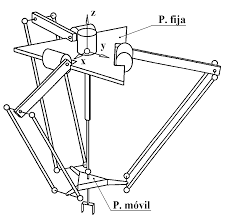
\includegraphics[scale=1.4]{imagenes/44.png} imagen 4.3
\end{center}
\begin{center}
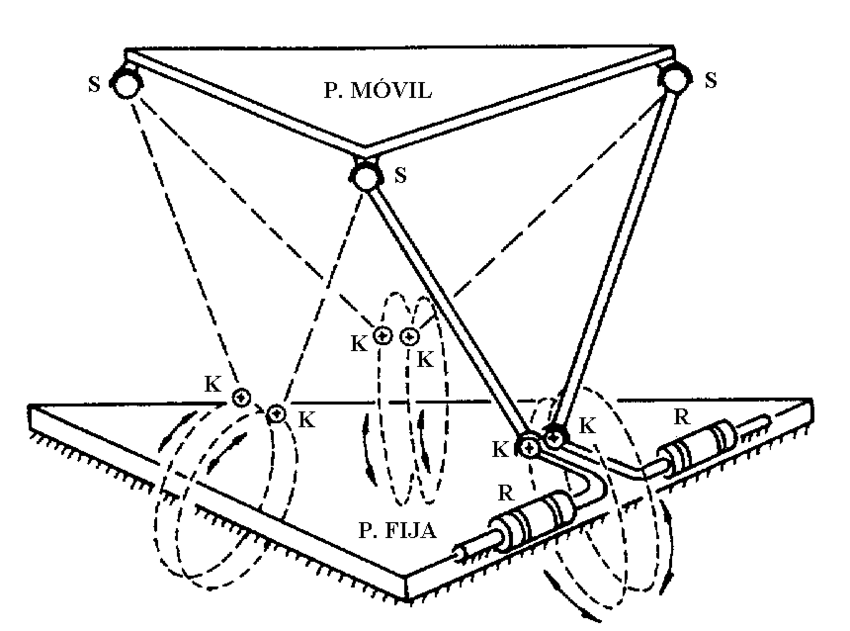
\includegraphics[scale=0.3]{imagenes/66.png} imagen 4.4
\end{center}

\textbf{Referencias}
@article{saravia2009revision,
  title={Revisi{\'o}n del estado del arte de manipuladores paralelos},
  author={Saravia, Darly Babeth P and Lopez, Marlon Jhair H and Riaza, Hector Fabio Q},
  journal={Scientia et technica},
  volume={2},
  number={42},
  pages={81--86},
  year={2009},
  publisher={Universidad Tecnol{\'o}gica de Pereira}
}


\end{document}